\documentclass{article}

% PACKAGES
\usepackage[margin=0.75in]{geometry}
\usepackage{amsmath}
\usepackage{amssymb}
\usepackage{graphicx}
\usepackage{subcaption}
\usepackage{float}

% TITLE
\title{Math 273A - Project 1}
\author{Eric Weise - A09642187}

\begin{document}
\maketitle

\subsection*{My code}
you can find my code at:
{\it  https://github.com/ericdweise/math-273a/blob/master/project1/project1.py}

\subsection*{Note}
In my convention, an $m\times n$ image has $m$ rows and $n$ columns. $m$ is the height, $n$ is the width.

\begin{figure}[H]
    \caption{Starting image}
    \centering
        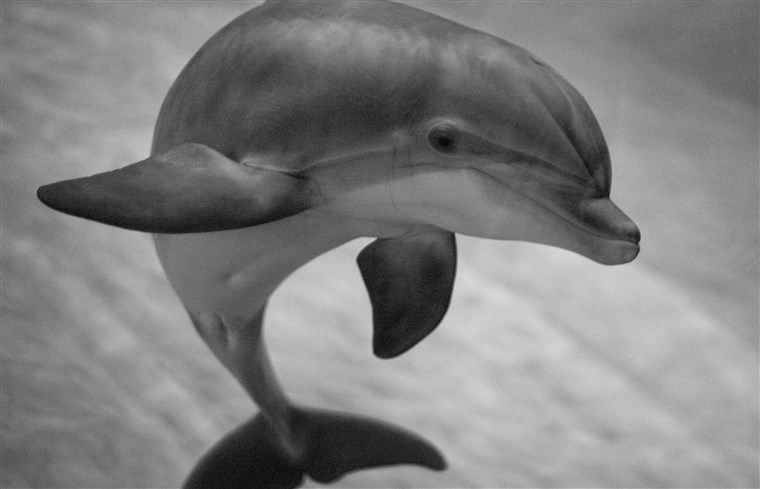
\includegraphics[width=0.5\textwidth]{part-0.png}
\end{figure}


\newpage
\section*{Part A}
\begin{figure}[H]
    \caption{Image resized to 1000$\times$1000 pixels}
    \centering
        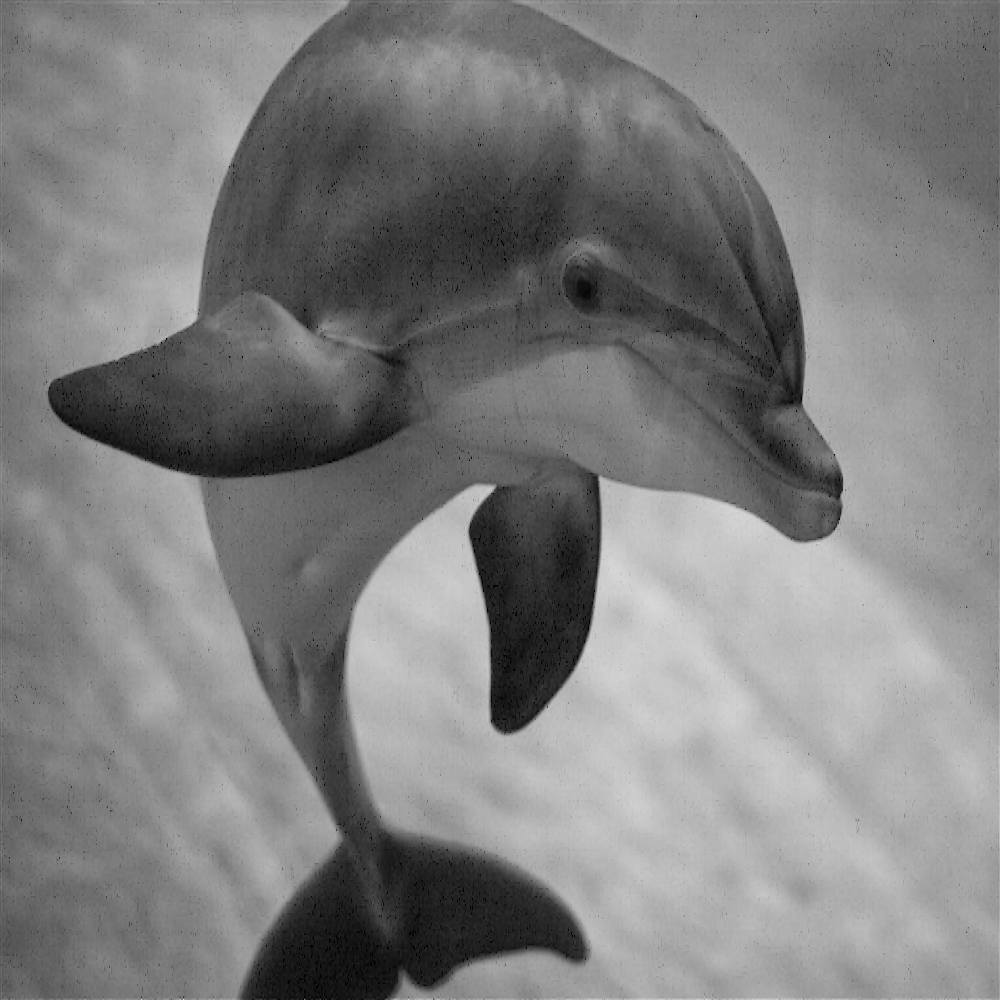
\includegraphics[width=0.5\textwidth]{part-a.png}
\end{figure}



\newpage
\section*{Part B}
\begin{figure}[H]
    \caption{Image resized to 760$\times$489 pixels}
    \centering
        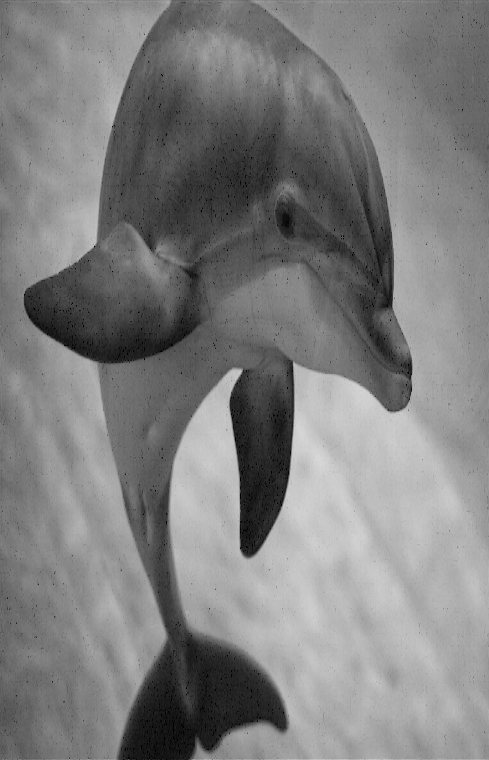
\includegraphics[width=0.5\textwidth]{part-b.png}
\end{figure}



\newpage
\section*{Part C}
\begin{figure}[H]
    \caption{Image resized to 100$\times$300 pixels}
    \centering
        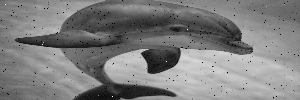
\includegraphics[width=0.5\textwidth]{part-c.png}
\end{figure}

\end{document}
